\chapteropen{Chapter 6: Software Requirements Specification}{chapter-6}
\markboth{Ch. 6 | SRS}{}


\begin{studycolumns}
\vspace{0pt}
\begin{eli5box}
An SRS is an agreement about the cake you ordered: size, flavour, delivery and how to check it. It should not secretly replace your order with the baker's preferred recipe. Someone reading the agreement should be able to tell whether the delivered product meets it.
\end{eli5box}
\textbf{Answer check:} Specify required behaviour, interfaces and qualities; leave arbitrary design choices out. Use identifiers plus trace links, measurable conditions and explicit TBDs. Adding ``shall'' alone does not repair an ambiguous requirement.
\end{studycolumns}

\subsection*{Visual: see the SRS as five compartments}
\sectionlabel{h-visual-see-the-srs-as-five-compartments}


\par\smallskip\noindent\begin{minipage}{\linewidth}\centering
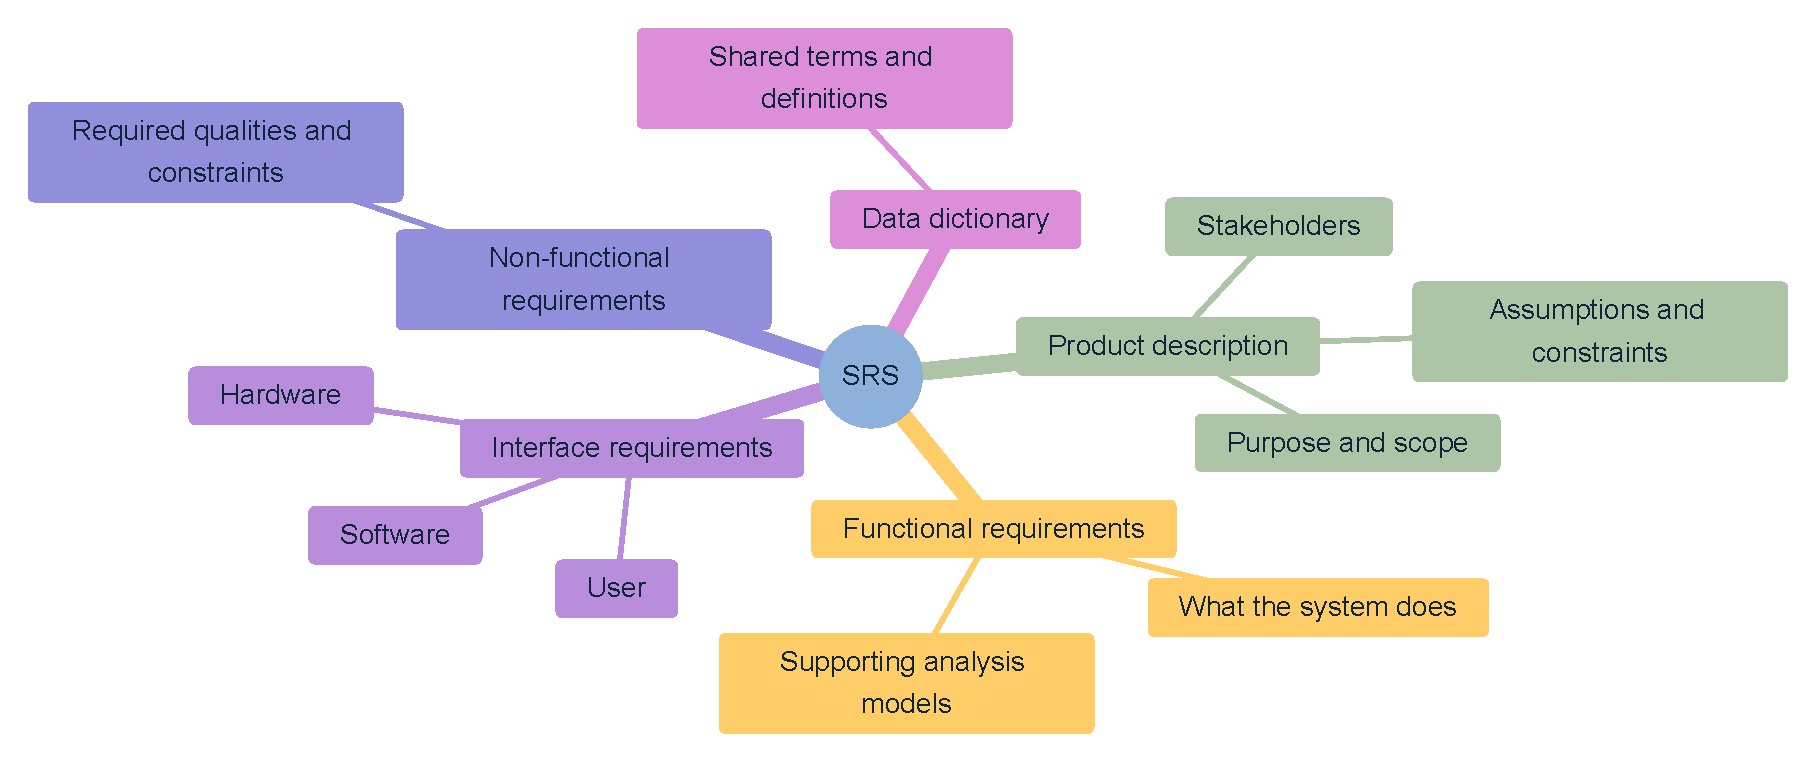
\includegraphics[width=514.00pt]{images/fig-021.pdf}
\captionof{figure}{see the SRS as five compartments}\end{minipage}\par\smallskip

\begin{studycolumns}
\vspace{0pt}



\needspace{4\baselineskip}
\subsection*{6.1 What the SRS is (six definitions that get paraphrased into exam questions)}
\sectionlabel{h-61-what-the-srs-is-six-definitions-that-get-paraphrased-into-exam-questions}
\begin{enumerate}
\item The \textbf{output of requirements elicitation and analysis}.
\item An organisation's \textbf{written understanding} of a customer's requirements and dependencies at a point in time, prior to design/\allowbreak{}development.
\item A \textbf{two-way insurance policy}: both client and organisation understand each other's requirements.
\item A statement in \textbf{precise, clear language} of the functions and capabilities the system must provide, plus required constraints.
\item A \textbf{blueprint} for completing the project with as little cost growth as possible.
\item \textbf{Detailed functional and non-functional requirements --- it does NOT contain design suggestions.}
\end{enumerate}
\needspace{4\baselineskip}
\subsection*{6.2 Purpose of the SRS (4 items)}
\sectionlabel{h-62-purpose-of-the-srs-4-items}
\begin{enumerate}
\item Give the customer assurance that the organisation understands the problems to be solved and the necessary software behaviour.
\item \textbf{Decompose} the problem into component parts.
\item Serve as \textbf{input to the design specification} --- so it must contain sufficient functional detail for a design solution to be devised.
\item Serve as the \textbf{parent/\allowbreak{}master document for testing and validation}.
\end{enumerate}
\end{studycolumns}

\Needspace{4\baselineskip}
\subsection*{6.3 Contents (5 sections --- memorise the numbering)}
\sectionlabel{h-63-contents-5-sections--memorise-the-numbering}


{\fontsize{9}{11}\selectfont
\begin{longtable}{L{\dimexpr 0.08684\linewidth-2.08pt\relax}L{\dimexpr 0.28102\linewidth-6.74pt\relax}L{\dimexpr 0.63214\linewidth-15.17pt\relax}}
\toprule
\rowcolor{ice}\textbf{Section } & \textbf{Section} & \textbf{Contents} \\
\midrule\endfirsthead
\toprule\rowcolor{ice}\textbf{Section } & \textbf{Section} & \textbf{Contents} \\
\midrule\endhead
\multicolumn{3}{r}{\scriptsize Continued on next page}\\\endfoot
\bottomrule\endlastfoot
1 & \textbf{Product description} & a) Purpose of the system (mission statement) \ensuremath{\cdot} b) Scope \ensuremath{\cdot} c) Users and stakeholders \ensuremath{\cdot} d) Assumptions and constraints \\
2 & \textbf{Functional requirements} & Precise numbered statements + activity diagrams, use case diagrams with descriptions, class diagrams, sequence diagrams, communication diagrams, state machine diagrams, UI prototype \\
3 & \textbf{Non-functional requirements} & Numbered statements covering performance, standards, reliability, availability, security, maintainability, portability \\
4 & \textbf{Interface requirements} & a) \textbf{User} (screen formats, layouts, report/\allowbreak{}menu content, function keys) \ensuremath{\cdot} b) \textbf{Hardware} (ports, instruction sets) \ensuremath{\cdot} c) \textbf{Software} (interfaces to DBMS, OS, maths packages) \\
5 & \textbf{Data dictionary} & Unambiguously defines all terms, phrases and abbreviations used in the SRS \\
\end{longtable}
}

Standards reference: \textbf{IEEE 830-1998}, \emph{IEEE Recommended Practice for Software Requirements Specifications}.

Who writes it: it should be in \textbf{natural language, unambiguous, with diagrams as necessary}; it must be understood by the development team; programmers/\allowbreak{}managers are seldom the best writers, so it is good practice to \textbf{involve a technical writer}.


\Needspace{4\baselineskip}
\subsection*{6.4 The nine language-quality characteristics}
\sectionlabel{h-64-the-nine-language-quality-characteristics}


{\fontsize{9}{11}\selectfont
\begin{longtable}{L{\dimexpr 0.11235\linewidth-2.70pt\relax}L{\dimexpr 0.28057\linewidth-6.73pt\relax}L{\dimexpr 0.60708\linewidth-14.57pt\relax}}
\toprule
\rowcolor{ice}\textbf{\#} & \textbf{Characteristic} & \textbf{Test you can apply} \\
\midrule\endfirsthead
\toprule\rowcolor{ice}\textbf{\#} & \textbf{Characteristic} & \textbf{Test you can apply} \\
\midrule\endhead
\multicolumn{3}{r}{\scriptsize Continued on next page}\\\endfoot
\bottomrule\endlastfoot
1 & \textbf{Correct} & Only user representatives can confirm; include them in inspections \\
2 & \textbf{Feasible} & Implementable within known capabilities/\allowbreak{}limits of system and environment \\
3 & \textbf{Necessary} & Can you identify its origin (customer need, external interface, standard)? If not, maybe not necessary \\
4 & \textbf{Unambiguous} & Multiple readers must reach \textbf{one} interpretation \\
5 & \textbf{Verifiable} & Can you devise a test /\allowbreak{} inspection /\allowbreak{} demonstration for it? \\
6 & \textbf{Complete} & Nothing missing; organise hierarchically so reviewers can spot gaps \\
7 & \textbf{Consistent} & No conflict with other requirements or higher-level requirements \\
8 & \textbf{Modifiable} & Uniquely labelled, expressed separately, change history maintained \\
9 & \textbf{Traceable} & Link each requirement to its source and its realisation \\
\end{longtable}
}

\begin{studycolumns}
\vspace{0pt}

\needspace{4\baselineskip}
\subsection*{6.5 Word list (memorise both columns)}
\sectionlabel{h-65-word-list-memorise-both-columns}
\textbf{YES Use these words}


\begin{referenceentries}
\textit{\textbf{YES Use} / \textbf{Meaning}}\par\smallskip
\noindent \textbf{\textbf{Shall}}: Dictates provision of a functional capability\par
\noindent \textbf{\textbf{Must /\allowbreak{} Must not}}: Establishes performance requirement or constraint\par
\noindent \textbf{\textbf{Is required to}}: Imperative in SRS statements\par
\noindent \textbf{\textbf{Are applicable}}: Includes standards/\allowbreak{}documentation by reference\par
\noindent \textbf{\textbf{Responsible for}}: Imperative for pre-defined architectures\par
\noindent \textbf{\textbf{Will}}: Cites what the operational/\allowbreak{}development \textbf{environment} will provide\par
\end{referenceentries}
\textbf{NO Avoid these words}


\begin{referenceentries}
\textit{\textbf{NO Avoid} / \textbf{Why}}\par\smallskip
\noindent \textbf{adequate}: vague threshold\par
\noindent \textbf{as a minimum}: unbounded\par
\noindent \textbf{be capable of\ldots{}}: avoids commitment\par
\noindent \textbf{as applicable /\allowbreak{} as appropriate}: optional\par
\noindent \textbf{effective}: unmeasurable\par
\noindent \textbf{if possible /\allowbreak{} if practical}: optional\par
\noindent \textbf{timely}: unmeasurable\par
\noindent \textbf{normal}: undefined baseline\par
\end{referenceentries}

\begin{quote}\small\color{navy}
The two lists are \textbf{independent} --- the lecture presents them side by side, so a row on the left is not the "opposite" of the row on the right.

\end{quote}

\begin{quote}\small\color{navy}
\textbf{Trap (shall vs will).} \textbf{Shall} binds the \emph{system}; \textbf{will} describes what the \emph{environment} supplies. "The system \textbf{shall} \ldots{}" is a requirement; "The user \textbf{will} provide a valid card" is an assumption about the environment. Swapping them blurs responsibility for the behaviour.


\end{quote}
\end{studycolumns}
